\documentclass[]{article}

\usepackage[utf8]{inputenc}
\usepackage[usenames,dvipsnames]{xcolor}
\usepackage{fullpage}
\usepackage[upright]{fourier}
\usepackage{tkz-graph}
\usetikzlibrary{arrows}

\usepackage[paperheight=5.95in,paperwidth=7.5in,margin=0in]{geometry}


\begin{document}
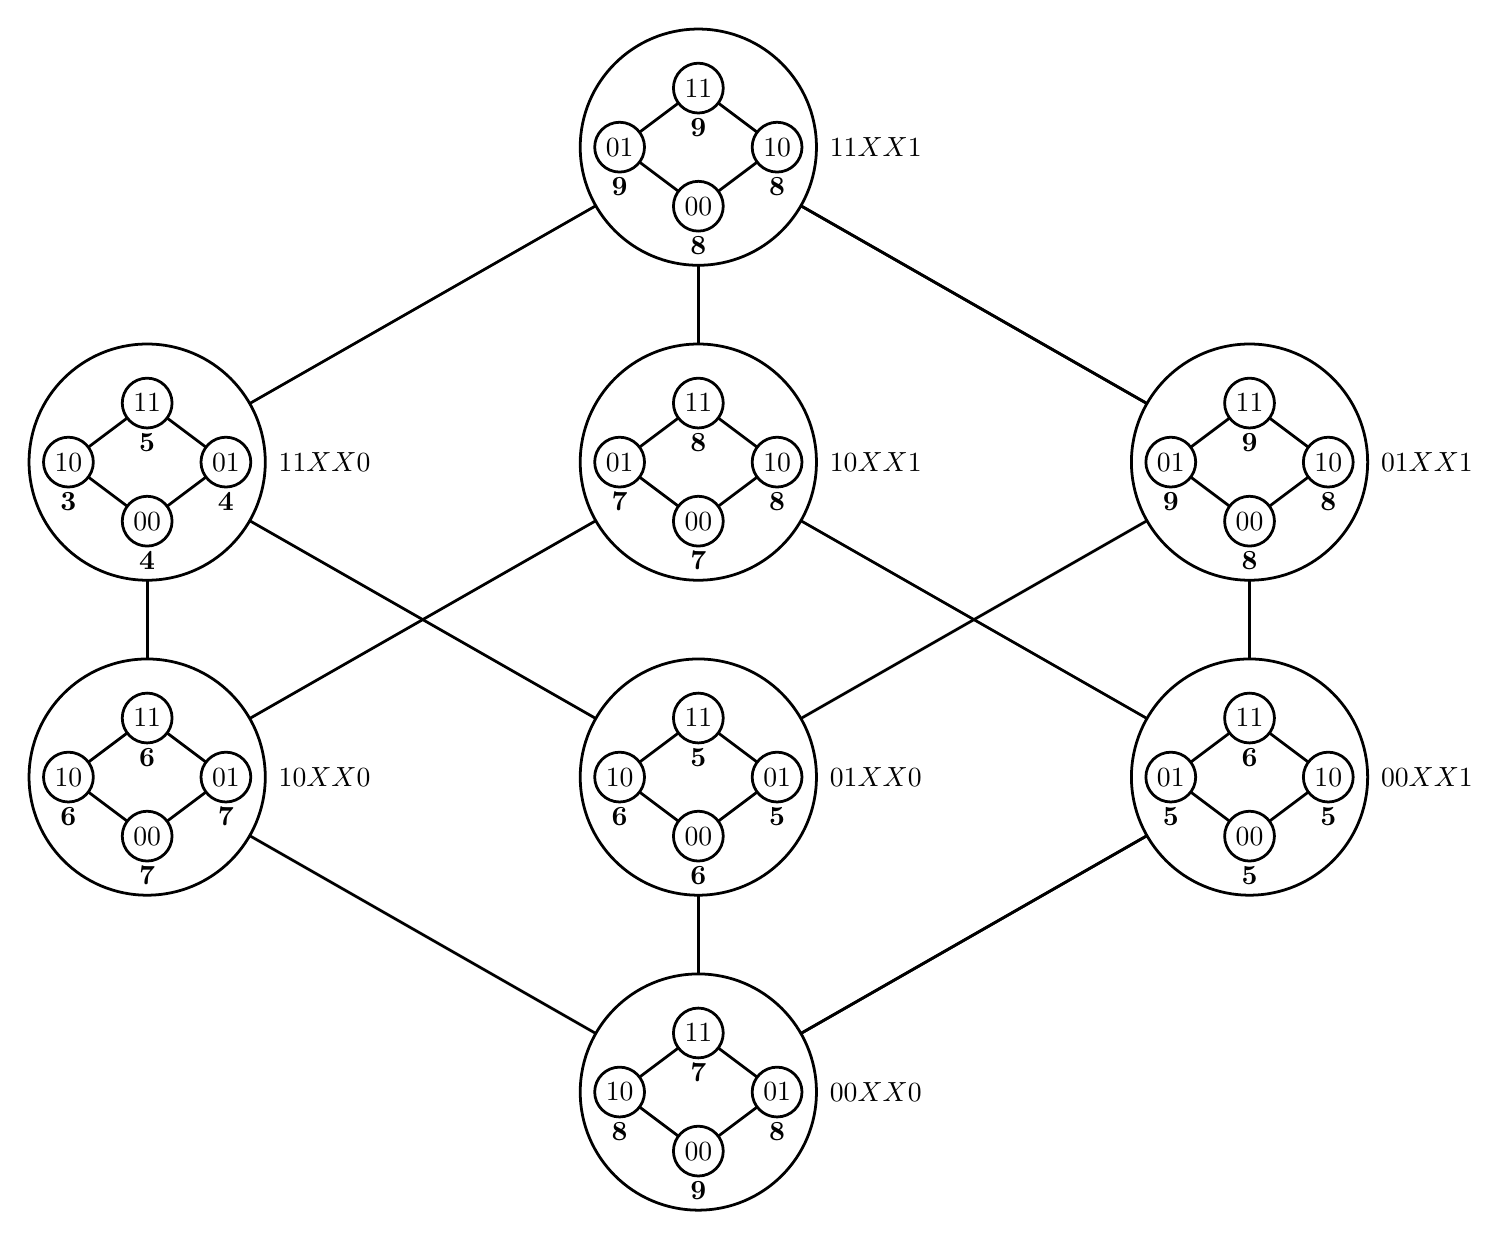
\begin{tikzpicture}

  \SetVertexNormal[Shape      = circle,
                   FillColor  = white,
                  LineWidth  = 1pt]

  \SetUpEdge[lw         = 1pt,
             color      = black,
             labelcolor = white,
             labeltext  = my_red,
             labelstyle = {sloped,draw,text=my_blue}]

\Vertex[x=0, y=0, LabelOut=true, Ldist=35pt]{$00XX0$}
\Vertex[x=0, y=0]{$ $}

\Vertex[x=-7, y=4, LabelOut=true, Ldist=35pt]{$10XX0$}
\Vertex[x=-7, y=4]{$a$} 

\Vertex[x=0, y=4, LabelOut=true, Ldist=35pt]{$01XX0$}

\Vertex[x=0, y=4]{$b$}

\Vertex[x=7, y=4, LabelOut=true, Ldist=35pt]{$00XX1$}
\Vertex[x=7, y=4]{$c$}

% level 2

\Vertex[x=-7, y=8, LabelOut=true, Ldist=35pt]{$11XX0$}
\Vertex[x=-7, y=8]{$ab$}

\Vertex[x=0, y=8, LabelOut=true, Ldist=35pt]{$10XX1$}
\Vertex[x=0, y=8]{$ac$} 

\Vertex[x=7, y=8, LabelOut=true, Ldist=35pt]{$01XX1$}
\Vertex[x=7, y=8]{$bc$}

% level 3

\Vertex[x=0, y=12, LabelOut=true, Ldist=35pt]{$11XX1$}
\Vertex[x=0, y=12]{$abc$}


\SetUpEdge[lw = 1pt]
\tikzset{EdgeStyle/.style={-}}
     \Edges($ $, $c$) 
     \Edges($c$, $bc$) 
     \Edges($bc$, $abc$) 


     \Edges($ $, $a$) 
     \Edges($ $, $b$) 
     \Edges($ $, $c$) 

     \Edges($a$, $ab$) 
     \Edges($a$, $ac$) 

     \Edges($b$, $ab$) 
     \Edges($b$, $bc$) 

     \Edges($c$, $ac$) 
     \Edges($c$, $bc$) 

     \Edges($abc$, $ac$) 
     \Edges($abc$, $bc$) 
     \Edges($abc$, $ab$) 



% level 1

\draw [line width = 1pt, color=black, fill=white] (0, 0) circle (15mm);  % empty set
\Vertex[x=-1, y=0, L=$10$]{00XX0$10$} 
\node  at (-1, -0.5) (c00XX0$10$) {\bf 8};
\Vertex[x=1, y=0, L=$01$]{00XX0$01$} 
\node  at (1, -0.5) (c00XX0$01$) {\bf 8};
\Vertex[x=0, y=0.75, L=$11$]{00XX0$11$} 
\node  at (0, 0.25) (c00XX0$11$) {\bf 7};
\Vertex[x=0, y=-0.75, L=$00$]{00XX0$00$} 
\node  at (0, -1.25) (c00XX0$00$) {\bf 9};
\Edges(00XX0$10$,00XX0$00$)
\Edges(00XX0$01$,00XX0$00$)
\Edges(00XX0$10$,00XX0$11$)
\Edges(00XX0$11$,00XX0$01$)


% level 2

\draw [line width = 1pt, color=black, fill=white] (-7, 4) circle (15mm);  % a
\Vertex[x=-8, y=4, L=$10$]{10XX0$10$} 
\node  at (-8, 3.5) (c10XX0$10$) {\bf 6};
\Vertex[x=-6, y=4, L=$01$]{10XX0$01$} 
\node  at (-6, 3.5) (c10XX0$01$) {\bf 7};
\Vertex[x=-7, y=4.75, L=$11$]{10XX0$11$} 
\node  at (-7, 4.25) (c10XX0$11$) {\bf 6};
\Vertex[x=-7, y=3.25, L=$00$]{10XX0$00$} 
\node  at (-7, 2.75) (c10XX0$00$) {\bf 7};
\Edges(10XX0$10$,10XX0$00$)
\Edges(10XX0$01$,10XX0$00$)
\Edges(10XX0$10$,10XX0$11$)
\Edges(10XX0$11$,10XX0$01$)


\draw [line width = 1pt, color=black, fill=white] (0, 4) circle (15mm);  % b
\Vertex[x=-1, y=4, L=$10$]{01XX0$10$} 
\node  at (-1, 3.5) (c01XX0$10$) {\bf 6};
\Vertex[x=1, y=4, L=$01$]{01XX0$01$} 
\node  at (1, 3.5) (c01XX0$01$) {\bf 5};
\Vertex[x=0, y=4.75, L=$11$]{01XX0$11$} 
\node  at (0, 4.25) (c01XX0$11$) {\bf 5};
\Vertex[x=0, y=3.25, L=$00$]{01XX0$00$} 
\node  at (0, 2.75) (c01XX0$00$) {\bf 6};
\Edges(01XX0$10$,01XX0$00$)
\Edges(01XX0$01$,01XX0$00$)
\Edges(01XX0$10$,01XX0$11$)
\Edges(01XX0$11$,01XX0$01$)


\draw [line width = 1pt, color=black, fill=white] (7, 4) circle (15mm);  % c
\Vertex[x=8, y=4, L=$10$]{00XX1$10$} 
\node  at (8, 3.5) (c00XX1$10$) {\bf 5};
\Vertex[x=6, y=4, L=$01$]{00XX1$01$} 
\node  at (6, 3.5) (c00XX1$01$) {\bf 5};
\Vertex[x=7, y=4.75, L=$11$]{00XX1$11$} 
\node  at (7, 4.25) (c00XX1$11$) {\bf 6};
\Vertex[x=7, y=3.25, L=$00$]{00XX1$00$} 
\node  at (7, 2.75) (c00XX1$00$) {\bf 5};
\Edges(00XX1$10$,00XX1$00$)
\Edges(00XX1$01$,00XX1$00$)
\Edges(00XX1$10$,00XX1$11$)
\Edges(00XX1$11$,00XX1$01$)

% level 3

\draw [line width = 1pt, color=black, fill=white] (-7, 8) circle (15mm);  % ab
\Vertex[x=-8, y=8, L=$10$]{11XX0$10$} 
\node  at (-8, 7.5) (c11XX0$10$) {\bf 3};
\Vertex[x=-6, y=8, L=$01$]{11XX0$01$} 
\node  at (-6, 7.5) (c11XX0$01$) {\bf 4};
\Vertex[x=-7, y=8.75, L=$11$]{11XX0$11$} 
\node  at (-7, 8.25) (c11XX0$11$) {\bf 5};
\Vertex[x=-7, y=7.25, L=$00$]{11XX0$00$} 
\node  at (-7, 6.75) (c11XX0$00$) {\bf 4};
\Edges(11XX0$10$,11XX0$00$)
\Edges(11XX0$01$,11XX0$00$)
\Edges(11XX0$10$,11XX0$11$)
\Edges(11XX0$11$,11XX0$01$)

\draw [line width = 1pt, color=black, fill=white] (0, 8) circle (15mm);  % ac
\Vertex[x=1, y=8, L=$10$]{10XX1$10$} 
\node  at (1, 7.5) (c10XX1$10$) {\bf 8};
\Vertex[x=-1, y=8, L=$01$]{10XX1$01$} 
\node  at (-1, 7.5) (c10XX1$01$) {\bf 7 };
\Vertex[x=0, y=8.75, L=$11$]{10XX1$11$} 
\node  at (0, 8.25) (c10XX1$11$) {\bf 8};
\Vertex[x=0, y=7.25, L=$00$]{10XX1$00$} 
\node  at (0, 6.75) (c10XX1$00$) {\bf 7};
\Edges(10XX1$10$,10XX1$00$)
\Edges(10XX1$01$,10XX1$00$)
\Edges(10XX1$10$,10XX1$11$)
\Edges(10XX1$11$,10XX1$01$)

\draw [line width = 1pt, color=black, fill=white] (7, 8) circle (15mm);  % bc
\Vertex[x=8, y=8, L=$10$]{01XX1$10$} 
\node  at (8, 7.5) (c01XX1$10$) {\bf 8};
\Vertex[x=6, y=8, L=$01$]{01XX1$01$} 
\node  at (6, 7.5) (c01XX1$01$) {\bf 9};
\Vertex[x=7, y=8.75, L=$11$]{01XX1$11$} 
\node  at (7, 8.25) (c01XX1$11$) {\bf 9};
\Vertex[x=7, y=7.25, L=$00$]{01XX1$00$} 
\node  at (7, 6.75) (c01XX1$00$) {\bf 8};
\Edges(01XX1$10$,01XX1$00$)
\Edges(01XX1$01$,01XX1$00$)
\Edges(01XX1$10$,01XX1$11$)
\Edges(01XX1$11$,01XX1$01$)


% level 4

\draw [line width = 1pt, color=black, fill=white] (0, 12) circle (15mm);  % abc
\Vertex[x=1, y=12, L=$10$]{11XX1$10$} 
\node  at (1, 11.5) (c11XX1$10$) {\bf 8};
\Vertex[x=-1, y=12, L=$01$]{11XX1$01$} 
\node  at (-1, 11.5) (c11XX1$01$) {\bf 9};
\Vertex[x=0, y=12.75, L=$11$]{11XX1$11$} 
\node  at (0, 12.25) (c11XX1$11$) {\bf 9};
\Vertex[x=0, y=11.25, L=$00$]{11XX1$00$} 
\node  at (0, 10.75) (c11XX1$00$) {\bf 8};
\Edges(11XX1$10$,11XX1$00$)
\Edges(11XX1$01$,11XX1$00$)
\Edges(11XX1$10$,11XX1$11$)
\Edges(11XX1$11$,11XX1$01$)

\end{tikzpicture}
\end{document}
